% Options for packages loaded elsewhere
\PassOptionsToPackage{unicode}{hyperref}
\PassOptionsToPackage{hyphens}{url}
\PassOptionsToPackage{dvipsnames,svgnames,x11names}{xcolor}
%
\documentclass[
  10pt,
]{article}
\usepackage{amsmath,amssymb}
\usepackage{lmodern}
\usepackage{iftex}
\ifPDFTeX
  \usepackage[T1]{fontenc}
  \usepackage[utf8]{inputenc}
  \usepackage{textcomp} % provide euro and other symbols
\else % if luatex or xetex
  \usepackage{unicode-math}
  \defaultfontfeatures{Scale=MatchLowercase}
  \defaultfontfeatures[\rmfamily]{Ligatures=TeX,Scale=1}
\fi
% Use upquote if available, for straight quotes in verbatim environments
\IfFileExists{upquote.sty}{\usepackage{upquote}}{}
\IfFileExists{microtype.sty}{% use microtype if available
  \usepackage[]{microtype}
  \UseMicrotypeSet[protrusion]{basicmath} % disable protrusion for tt fonts
}{}
\makeatletter
\@ifundefined{KOMAClassName}{% if non-KOMA class
  \IfFileExists{parskip.sty}{%
    \usepackage{parskip}
  }{% else
    \setlength{\parindent}{0pt}
    \setlength{\parskip}{6pt plus 2pt minus 1pt}}
}{% if KOMA class
  \KOMAoptions{parskip=half}}
\makeatother
\usepackage{xcolor}
\usepackage[margin=1in]{geometry}
\usepackage{longtable,booktabs,array}
\usepackage{calc} % for calculating minipage widths
% Correct order of tables after \paragraph or \subparagraph
\usepackage{etoolbox}
\makeatletter
\patchcmd\longtable{\par}{\if@noskipsec\mbox{}\fi\par}{}{}
\makeatother
% Allow footnotes in longtable head/foot
\IfFileExists{footnotehyper.sty}{\usepackage{footnotehyper}}{\usepackage{footnote}}
\makesavenoteenv{longtable}
\usepackage{graphicx}
\makeatletter
\def\maxwidth{\ifdim\Gin@nat@width>\linewidth\linewidth\else\Gin@nat@width\fi}
\def\maxheight{\ifdim\Gin@nat@height>\textheight\textheight\else\Gin@nat@height\fi}
\makeatother
% Scale images if necessary, so that they will not overflow the page
% margins by default, and it is still possible to overwrite the defaults
% using explicit options in \includegraphics[width, height, ...]{}
\setkeys{Gin}{width=\maxwidth,height=\maxheight,keepaspectratio}
% Set default figure placement to htbp
\makeatletter
\def\fps@figure{htbp}
\makeatother
\setlength{\emergencystretch}{3em} % prevent overfull lines
\providecommand{\tightlist}{%
  \setlength{\itemsep}{0pt}\setlength{\parskip}{0pt}}
\setcounter{secnumdepth}{-\maxdimen} % remove section numbering
\newlength{\cslhangindent}
\setlength{\cslhangindent}{1.5em}
\newlength{\csllabelwidth}
\setlength{\csllabelwidth}{3em}
\newlength{\cslentryspacingunit} % times entry-spacing
\setlength{\cslentryspacingunit}{\parskip}
\newenvironment{CSLReferences}[2] % #1 hanging-ident, #2 entry spacing
 {% don't indent paragraphs
  \setlength{\parindent}{0pt}
  % turn on hanging indent if param 1 is 1
  \ifodd #1
  \let\oldpar\par
  \def\par{\hangindent=\cslhangindent\oldpar}
  \fi
  % set entry spacing
  \setlength{\parskip}{#2\cslentryspacingunit}
 }%
 {}
\usepackage{calc}
\newcommand{\CSLBlock}[1]{#1\hfill\break}
\newcommand{\CSLLeftMargin}[1]{\parbox[t]{\csllabelwidth}{#1}}
\newcommand{\CSLRightInline}[1]{\parbox[t]{\linewidth - \csllabelwidth}{#1}\break}
\newcommand{\CSLIndent}[1]{\hspace{\cslhangindent}#1}
\providecommand{\keywords}[1]{\textbf{Keywords:} #1}

\usepackage{pdflscape}
\newcommand{\blandscape}{\begin{landscape}}
\newcommand{\elandscape}{\end{landscape}}
\usepackage{fvextra}
\usepackage{float}
\usepackage{wrapfig}
\usepackage{amsmath}
\usepackage{threeparttable} %used to fix table with notes
\usepackage{float}
\usepackage{graphicx}
\usepackage{microtype}
\usepackage{setspace}
\usepackage[font=singlespacing]{caption}
\DefineVerbatimEnvironment{Highlighting}{Verbatim}{breaklines, commandchars=\\\{\}}
\DeclareMathOperator*{\argmax}{arg\,max}
\DeclareMathOperator*{\argmin}{arg\,min}
\singlespacing
\ifLuaTeX
  \usepackage{selnolig}  % disable illegal ligatures
\fi
\IfFileExists{bookmark.sty}{\usepackage{bookmark}}{\usepackage{hyperref}}
\IfFileExists{xurl.sty}{\usepackage{xurl}}{} % add URL line breaks if available
\urlstyle{same} % disable monospaced font for URLs
\hypersetup{
  pdftitle={Statistical Machine Learning for Listeria monocytogene Foodborne Disease Source Attribution},
  pdfauthor={Amos Okutse; Zexuan Yu; Rophence Ojiambo},
  colorlinks=true,
  linkcolor={blue},
  filecolor={Maroon},
  citecolor={Blue},
  urlcolor={blue},
  pdfcreator={LaTeX via pandoc}}

\title{Statistical Machine Learning for \emph{Listeria monocytogene} Foodborne Disease Source Attribution}
\author{Amos Okutse \and Zexuan Yu \and Rophence Ojiambo}
\date{15 December, 2022}

\begin{document}
\maketitle
\begin{abstract}
\textbf{Background:} Listeria remains one of the most severe contributors to foodborne disease burden due to the severity of its clinical manifestations. The role of statistical models in linking pathogenic isolates of listeria to a particular source remains substantially unexplored in outbreak investigations.

\textbf{Objectives:} To develop a statistical machine learning model for source attribution of \emph{Listeria monocytogene} pathogens to aid in foodborne illness source linkage in outbreak investigations.

\textbf{Methods:} Data from the National Center for Biotechnology Information (NCBI) pathogen detection database was used to derive a throughput model for listeria pathogen food source attribution. 10-fold cross validated and minority class up-sampled Naive Bayes and random forest models were fitted to the data for comparative purposes and to derive a robust model for food source attribution using n = 14653 pathogenic isolates.

\textbf{Results:} The average accuracy of the naive Bayes and random forest classification algorithms were 25.77\% (SE = 0.65\%) and 87.27\% (SE = 0.33\%), respectively, whereas the AUC values were 79.61\% (SE = 0.57\%) and 94.53\% (SE = 0.28\%) respectively. The random forest model showed the best performance and was used in listeria pathogen source attribution. The random forest model correctly linked 66.07\% of the pathogens to environmental sources (n = 5515 samples), 6.04\% to dairy and dairy products (n = 504 samples), 2.56\% to fruits (n = 214 samples), 0.50\% to humans (n = 42 samples), 0.45\% to leafy greens (n = 38 samples), 1.88\% to meat (n = 157 samples), 4.79\% to other unknown sources (n = 400 samples), 1.81\% to poultry (n = 151 samples), 1.48\% to sea food (n = 124 samples), and 2.85\% to vegetables (n = 238 samples).

\textbf{Conclusion and recommendations:} Statistical machine learning methods promise efficiency in source attribution of listeria pathogenic isolates which can substantially enhance the outbreak investigation process by reducing the possible pool of sources to be targeted by interventional policies. The government, risk managers and relevant departments can better predict and identify potential risks with this project. Additional validation should be carried out to enhance the usefulness and generalizability of the developed model for source attribution.
\end{abstract}

\singlespacing
\hspace{15pt} \keywords{Machine learning, Naive Bayes, Random forest, Food source attribution, \textit{Listeria monocytogene}, Predictive modeling, NCBI pathogen detection database}

\hypertarget{background}{%
\subsection{Background}\label{background}}

The burden of foodborne illnesses remains substantially high across the globe. Contaminated food has been implicated in 600 million incident cases of foodborne diseases and 420, 000 deaths per year worldwide with children below five years accounting for one-third of the total fatalities {[}\protect\hyperlink{ref-who2015}{1}{]}, {[}\protect\hyperlink{ref-Lee2021}{2}{]}. In the United States, foodborne illnesses result in about 128, 000 hospitalizations and about 3000 fatalities {[}\protect\hyperlink{ref-tanui2022machine}{3}{]}. Known pathogens account for most of the reported cases with most illnesses being caused by noroviruses (58\%), non-typhoid salmonella (11\%), \emph{Clostridium perfringens} (10\%), and \emph{Campylobacter SPP.} (9\%) whereas non-typhoid salmonella (35\%), and norovirus (26\%) account for the most hospitalizations {[}\protect\hyperlink{ref-Scallan2011}{4}{]}. \emph{Salmonella enterica}, \emph{E-coli}, and \emph{Listeria monocytogenes} remain the three most common pathogens linked to foodborne disease outbreaks, defined as two or more cases of a similar illness resulting from the ingestion of a common food {[}\protect\hyperlink{ref-tanui2022machine}{3}{]}, {[}\protect\hyperlink{ref-gourama2020foodborne}{5}{]}.

Despite its characterization with low morbidity, \emph{Listeria monocytogene} remains one of the most severe causes of foodborne-related disease burden, particularly, due to the severity of its clinical manifestations {[}\protect\hyperlink{ref-chlebicz2018campylobacteriosis}{6}{]}, {[}\protect\hyperlink{ref-filipello2020attribution}{7}{]}. The immuno-compromised, the elderly, pregnant women, and infants remain at high risk of listeriosis, a foodborne illness ranked as the third top cause of foodborne illness-associated deaths in the US {[}\protect\hyperlink{ref-lomonaco2015evolution}{8}{]}. The US Centers for Disease Control and Prevention (CDC) notes that about 1600 cases of listeriosis are recorded annually with about 260 mortalities {[}\protect\hyperlink{ref-cdc2022}{9}{]}. Outbreak investigations have shown links between these pathogens and specific food sources, a crucial phenomenon in identifying potential areas of food safety concerns including points of contamination and the current performance of foodborne illness prevention strategies {[}\protect\hyperlink{ref-tanui2022machine}{3}{]}. Many foodborne listeriosis outbreaks have been linked to a variety of foods, but mostly to different types of meat {[}\protect\hyperlink{ref-matle2020review}{10}{]}, {[}\protect\hyperlink{ref-hilliard2018genomic}{11}{]}. The first laboratory-confirmed outbreak of listeriosis associated with meat products was caused by contaminated turkeys in 1988 {[}\protect\hyperlink{ref-schwartz1989investigation}{12}{]}. Since then, most meat products have been associated with outbreaks or sporadic listeriosis, including processed vacuum-packed meat products {[}\protect\hyperlink{ref-chen2017prevalence}{13}{]} and sausage {[}\protect\hyperlink{ref-jensen2016molecular}{14}{]} among others. Similarly, contaminated non-meat foods including ice cream, and diced celery have been previously linked to outbreaks {[}\protect\hyperlink{ref-gaul2013hospital}{15}{]}, {[}\protect\hyperlink{ref-pouillot2016infectious}{16}{]}. In recent years, sporadic outbreaks of listeria have also been increasingly reported in developing countries across the globe {[}\protect\hyperlink{ref-de2014global}{17}{]}.

Technological advancements have seen increased attempts in leveraging the power of machine learning methods and core genome multilocus sequence typing (cgMLST) in the corroboration of epidemiological findings on food source attribution, in addition, to auditing the effect of public health interventions targeting the food chain on the food reservoirs {[}\protect\hyperlink{ref-tanui2022machine}{3}{]}, {[}\protect\hyperlink{ref-Munck2020}{18}{]}. This methodology enables differentiation of isolates and can be used to link them to their potential food sources in studies seeking to infer the food source of an outbreak given a pathogenic strain and ultimately result in a reduction in the incidence of foodborne illnesses {[}\protect\hyperlink{ref-Munck2020}{18}{]}. Since the pathogens associated with foodborne illnesses are prone to change, understanding the role of these changes in their adaptation to food handling practices is imperative in the effective surveillance of the distribution, as well as, the occurrence of the pathogens. Moreover, the use of genomic data with machine learning methods has gained precedence due to the ability of these methods to learn patterns in high-dimensional data sets which are then exploited in predictive models {[}\protect\hyperlink{ref-Munck2020}{18}{]}.

Even though machine learning models promise substantial gains in outbreak investigations, particularly while thinking about the role of genetic information in foodborne disease source attribution studies, there are a limited number of studies that have explored this avenue while thinking about the gains that these methods promise in allowing exploration of how foodborne pathogens adapt to or respond to food handling practices and how this information can be analyzed and ultimately reduce the incidence of listeriosis in humans. For instance, {[}\protect\hyperlink{ref-tanui2022machine}{3}{]} built a machine-learning model for food source attribution of Listeria monocytogenes using a boosted logit model whereas {[}\protect\hyperlink{ref-Njage2019}{19}{]} employed next-generation sequencing using support vector machines with linear kernels to predict the risk of illnesses. Additionally, Lupolova et al. {[}\protect\hyperlink{ref-lupolova2017patchy}{20}{]}, Munck et al. {[}\protect\hyperlink{ref-Munck2020}{18}{]}, Tanui et al. {[}\protect\hyperlink{ref-tanui2022machine}{3}{]}, and Karanth et al. {[}\protect\hyperlink{ref-karanth2022exploring}{21}{]} employed these methodologies in studying \emph{Salmonella enterica}. Varied statistical methods have been employed in analyzing foodborne disease outbreak dynamics. For listeria outbreaks, advanced statistical analysis methods have also come into play including studies by Liu et al. {[}\protect\hyperlink{ref-liu2021machine}{22}{]} and Vangay et al., {[}\protect\hyperlink{ref-vangay2014classification}{23}{]} which used machine learning methods to provide advice on listeria outbreaks. On the other hand, Sun et al. {[}\protect\hyperlink{ref-sun2019quantitative}{24}{]} used Markov chain Monte Carlo (MCMC) to simulate the risk of a Listeria outbreak whereas Pasonen et al. {[}\protect\hyperlink{ref-pasonen2019listeria}{25}{]} employed a repeated exposures model to assess the risk of a Listeria outbreak in Finnish fish products. Mughini-Gras et al. {[}\protect\hyperlink{ref-mughini2022statistical}{26}{]} conducted a meta-analysis of sporadic infection sources of some pathogens including Listeria based on the Bayesian framework whereas Lassen et al., {[}\protect\hyperlink{ref-lassen2016two}{27}{]} used whole genome sequencing to analyze the risk of listeria outbreaks.

Given the serious threat of foodborne diseases and the high burden posed by listeriosis on human health, this research investigation seeks to expand the literature on source attribution of human listeriosis pathogens by developing and proposing a throughput yet simple model for source attribution of listeriosis pathogens, leveraging the power of genetic information on these strains. We compare the performance of the Bayesian-based Naive Bayes classification algorithm and the ensemble-based random forest algorithm in linking listeriosis pathogens to a particular source with the goal of proposing a simple, robust, and suitable model for identifying a potential source of a listeriosis pathogen. A model for linking these pathogens to a likely source is crucial, not only in outbreak investigations and identifying potential areas of food safety concerns such as points of contamination and the current performance of foodborne illness prevention strategies {[}\protect\hyperlink{ref-tanui2022machine}{3}{]}, but also forms a way to audit the current performance of public health foodborne illness reduction strategies. The prevention of the transmission of foodborne illnesses promises substantial improvements in public health including reduction in the overall foodborne illness incidence and burden. Modeling periodic human cases of diseases attributable to food sources informs the public health decision making process including targeted interventions {[}\protect\hyperlink{ref-pires2014source}{28}{]}, {[}\protect\hyperlink{ref-Munck2020}{18}{]}.

\hypertarget{methodology}{%
\subsection{Methodology}\label{methodology}}

\hypertarget{data-source}{%
\subsubsection{Data source}\label{data-source}}

This study uses secondary data downloaded on the 18th October, 2022 from the National Center for Biotechnology Information (NCBI) Pathogen Detection database {[}\protect\hyperlink{ref-ncbi2016}{29}{]} which assimilates bacterial and fungal pathogen genomic sequences from sources including food, environment, and patient samples. The data are contributed by researchers and public health agencies who sequence samples and submit them to NCBI where the sequences are analyzed and compared to identify relations between sequences and thus aid the investigation of outbreaks including real-time surveillance of pathogens such as those for foodborne illnesses. The isolates present in the database were collected by 390 different institutions and organizations. Even though the NCBI pathogen detection allows real-time identification of clusters of related genomic sequences to aid in outbreak detection, and track the spread of resistance genes, a potential limitation of this data source is that it does not identify outbreaks or outbreak memberships, and analyses rely solely on publicly available data submitted to the database.

\begin{figure}[H]

{\centering 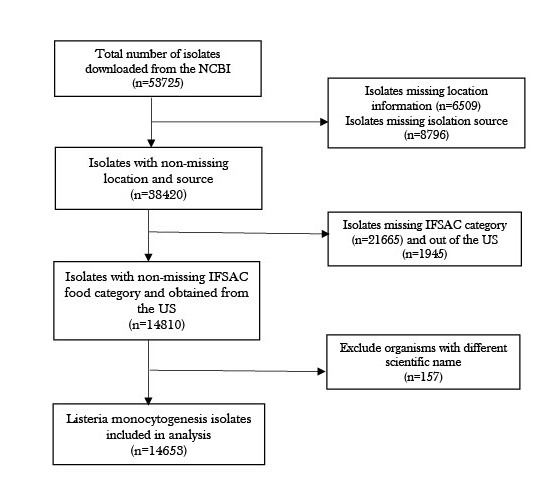
\includegraphics[width=0.86\linewidth]{../figures/data_cleaning} 

}

\caption{The flow of the data cleaning process based on the specified isolate inclusion criteria.}\label{fig:fig-one}
\end{figure}

\begin{table}[H]

\caption{\label{tab:table-one}Variable descriptions}
\centering
\begin{tabular}[t]{>{}l>{\raggedright\arraybackslash}p{11cm}}
\toprule
\textbf{Variable} & \textbf{Description}\\
\midrule
\textbf{Organism group} & The name of the taxonomy group that the isolate belongs to and is represented by the Genus species name, for our case we shall focus on Listeria monocytogenes.\\
\textbf{Isolate} & The unique Pathogen Detection accession of the isolate  where each accession has a prefix (PDT), which stands for Pathogen Detection Target.\\
\textbf{IFSAC category} & Categories of isolate sourcing information as developed by The Interagency Food Safety Analytics Collaboration (IFSAC).\\
\textbf{Isolation Source} & Provides information on the physical, environmental and/or local geographical source of the biological sample from which the sampled was derived.\\
\textbf{Isolation Type} & Contains categories of the isolation sources into either clinical or environmental/other groups.\\
\addlinespace
\textbf{Strain} & Denotes the microbial strain name used to distinguish a genetically distinct lineage separated from another strain by one or two mutations.\\
\textbf{Host} & Refers to the host species of the isolate such as Animal, Homo sapiens, Sheep, Pigeon, Horse and Guinea pig.\\
\textbf{Host Disease} & Host disease matches the identified isolate to a disease origin, for example Listeriosis, gastroenteritis, Meningitis and Septicaemia.\\
\textbf{Collection Date} & Gives the date the sample was collected.\\
\textbf{Create Date} & Gives the date on which the isolates were first seen by the Pathogen Detection system.\\
\addlinespace
\textbf{Outbreak} & Defines a way to group isolates that originated due to the same breakout among a specific group of people or within a specific area over a period of time.\\
\textbf{BioSample} & Describes the biological source materials used in experimental assay.\\
\textbf{Lat/Lon} & Provides the geographical coordinates (latitude and longitude) of the location where the sample was collected.\\
\textbf{Location} & Provides the geographical origin of the sample (Country or Region).\\
\textbf{Min-Same} & Represents the minimum single nucleotide polymorphism (SNP) distance to another isolate of the same isolation type for example, the minimum SNP distance from one clinical isolate to another clinical isolate.\\
\addlinespace
\textbf{Min Diff} & Represents the minimum SNP distance to another isolate of a different isolation type. For example, the minimum SNP difference from a clinical isolate to an environmental isolate.\\
\textbf{Serovar} & Represents the combined field of sub-species, serotype, or serovar\\
\textbf{AMR Genotypes} & Provides information on the antimicrobial resistance (AMR) genes found in each isolate.\\
\textbf{SNP Cluster} & Represents single nucleotide polymorphisms (SNP) clusters, where the genome assemblies are closely linked to each other.\\
\bottomrule
\end{tabular}
\end{table}

\hypertarget{data-and-variable-descriptions}{%
\subsubsection{Data and variable descriptions}\label{data-and-variable-descriptions}}

The downloaded data was comprised of n = 53, 725 \emph{Listeria monocytogenes} pathogens with 50 variables related to the pathogenic strains submitted, including information about who collected the isolate, its taxonomic name, its isolation source, date of collection (day, month, year), country or state from which the strain originated, among other metadata. Table \ref{tab:table-one} gives an overview of the variables considered in this analyses and their descriptions. Given the vast amount of information available in the database, these analyses employed an inclusion criteria to select strains for further analysis. In particular, for consideration and inclusion into the analysis sample, the isolate had to have a non-missing location, had been collected in the US, had a non-missing isolation source, and IFSAC category. The analysis sample based on this inclusion criteria included a total of n = 14, 653 \emph{Listeria monocytogenes} pathogens. Figure \ref{fig:fig-one} summarizes the isolate inclusion criteria for analysis and the resulting sample size.

\hypertarget{missing-data}{%
\subsubsection{Missing Data}\label{missing-data}}

We shall start by assessing the missingness in our data set. Figure \ref{fig:fig-two} shows us the overall missingness of our selected variables ordered from the least to the largest missing percentage. Key to note here is that there is over 86\% missing observations in the variables. \texttt{Host\ Disease}, \texttt{AST\ Phenotypes}, \texttt{Computed\ types}, \texttt{Virulence\ genotypes}, \texttt{Source\ type} and \texttt{Outbreak} have approximately 100\% of missing values. Variables such as \texttt{Isolation\ source}, \texttt{Isolation\ type}, \texttt{BioSample}, \texttt{Location}, \texttt{AMR\ genotypes} and \texttt{Isolates} have no missingness present. The missingness observed in this data set is likely due to under-reporting or non-response by the researchers or clinicians who submit this information on the NCBI website. Missing information in the collection date variable could be due to data entry errors when entering this information or just an oversight by the submitter. Generally, the missingness can be attributed to the high variations in the reporting practices or amount of time taken for lab processing prior to submission to the NCBI pathogen detection database. We acknowledge that this amount of missingness will be pose a major limitation in our study as these variables may not be informative in our analysis and may limit the interpretation and generalizability of our study findings. All analyses in the next sections consider a complete case analysis.

\begin{figure}[H]

{\centering 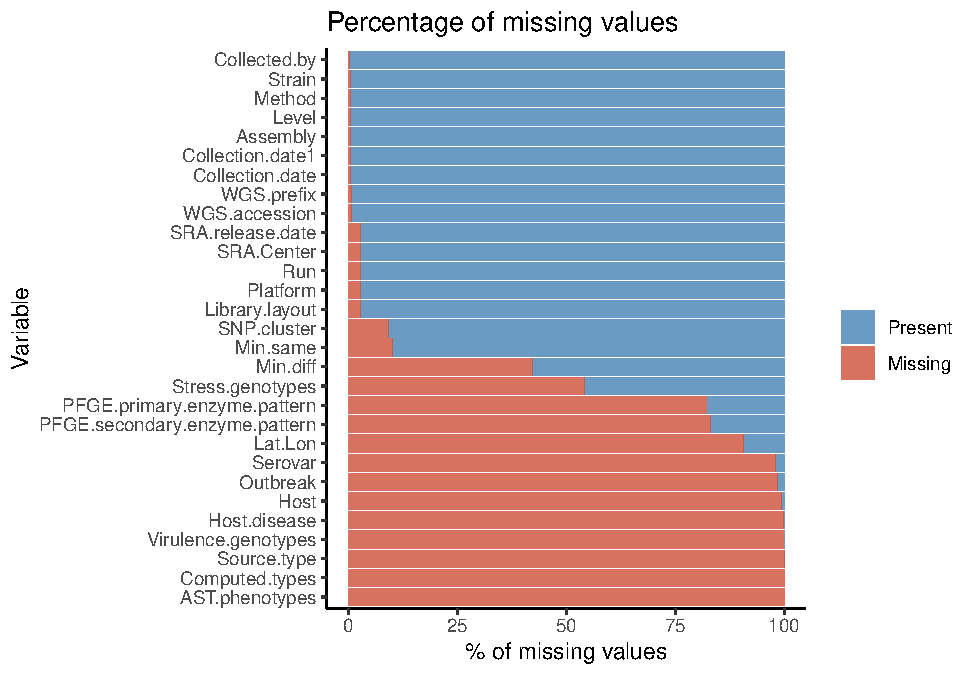
\includegraphics{php2550_final_manuscript_files/figure-latex/fig-two-1} 

}

\caption{Missing values in variables.}\label{fig:fig-two}
\end{figure}

\hypertarget{statistical-modeling}{%
\subsection{Statistical modeling}\label{statistical-modeling}}

We sought to compare the performance of the Bayesian-based Naive Bayes classification algorithm and the ensemble-based random forest algorithm in linking listeriosis pathogens to a particular source with the goal of proposing a simple and robust model for identifying a potential source associated with a listeriosis pathogen. A model for linking these pathogens to a likely source is crucial, in outbreak investigations, identifying potential areas of safety concerns, and auditing the current performance of foodborne illness prevention strategies, and ultimately in informing public health policy for listeriosis incidence reduction.

\hypertarget{statistical-learning-models}{%
\subsubsection{Statistical learning models}\label{statistical-learning-models}}

\textbf{1. Naïve Bayes}

The Naïve Bayes algorithm is a supervised machine learning technique for classification that uses a Bayesian-based approach under the \emph{naïve} assumption that features in a data set are independent of each of each other. The methodology proceeds by using conditional probability and the principles of the Bayes theorem to classify an input based on features present in a dataset. The Bayes theorem which forms a fundamental building block of the algorithm follows as:
\begin{equation}
    P(A|B) = \frac{P(B|A)P(A)}{P(B)}
\end{equation}
where \(A\) is the proposition, \(B\) is the evidence, \(P(A|B)\) denotes the posterior probability, \(P(B|A)\) denotes the likelihood, \(P(A)\) is the prior probability of event \(A\) and \(P(B)\) denotes the prior probability of the evidence, \(B\) {[}\protect\hyperlink{ref-gelman1995bayesian}{30}{]}.

In order for inferences to be made about the an unknown observation, the method proceeds by first building a distribution for the unknown observation unconditioned on the observed data, that is, the prior predictive distribution. Given the data have been observed, the prior predictive distribution is then updated to yield the posterior predictive distribution. The outcome, \(Y\) is often dependent on multiple features, \(p\) which can be denoted as \(\mathbf{X} = x_1, x_2, \cdots, x_p\) and one or more output classes, \(\mathbf{C} = C_1, C_2, \cdots, C_k\). The goal of the algorithm is to determine the conditional probability of an event with features, \(\mathbf{X}\) belonging to a class, \(C_k\). Based on the Bayes theorem, these can be written as:
\begin{equation}
    P(C_k|\mathbf{X}) = \frac{P(C_k)P(\mathbf{X}|C_k)}{P(\mathbf{X})}
\end{equation}

The Naive Bayes algorithm allots a class label \(\hat{y} = C_k\) for some \(k\) and is defined as:
\begin{equation}
    \hat{y} = \mathop{\mathrm{arg\,max}}_{k \in \{1, \cdots, k\}} P(C_k) \prod_{i = 1}^{p} P(x_i|C_k)
\end{equation}

The suitability of this algorithm for our particular analyses followed from our interest in perform multi-class and potentially, multi-label classification. The algorithm is easy to implement, is relatively fast to train and in classifying unknown individuals, and has been shown to perform relatively well with minimal to no hyper-parameter tuning when compared with other algorithms. Additionally, the algorithm uses evidence to update the estimation of the posterior and is robust {[}\protect\hyperlink{ref-Chen2021}{31}{]}.

\textbf{2. Random forests}

Random forests are an ensemble of multiple decision trees which employ bagging to reduce over-fitting and thus enhance the generalizability of the resulting model. Multiple trees are fitted on the training data using randomly selected predictors to ensure that the resulting trees are uncorrelated. In training each tree, some samples are not used in the training process and are used in the estimation of the model performance by averaging. Each of the trees building up the random forest makes its prediction/classification to results in multiple predictions which are then averaged to inform the final result. Random forests adopt the bagging methodology which involves creating sub-samples (or replicates), \(B\) of the original data with replacement. The model is then fitted on each bootstrap sample, \(b = 1, 2, \cdots, B\) obtaining a prediction, \(\hat{f}^{*b}(x)\). The final result follows from averaging all the model predictions in the context of a regression problem or majority voting for classification problems where one of the models with the most common (classification) result is chosen at random {[}\protect\hyperlink{ref-James2013}{32}{]}. The bagging estimate is defined as

\begin{align}
    \begin{split}
        \hat{f}(x)^{\textrm{bag}} &= \frac{1}{B} \sum_{b=1}^{B} \hat{f}^{*ab}(x) \\
        & \textrm{where} ~ B ~ \textrm{denotes the number of bootstrap samples} \\
        & \textrm{and} ~ \hat{f}^{*ab}(x) ~ \textrm{denotes the m$^{th}$ model's prediction} \\
    \end{split}
\end{align}

Bootstrap aggregating provides a natural way of estimating the generalizability of the model on unseen data since the fitted models on the bootstrapped samples use only a portion of the observations in training such that the remaining portion of the data not used in fitting the bagged tree (i.e.~Out Of Bag {[}OOB{]}) can be used in estimating the performance of the model by using these OOB observations to calculate the OOB error {[}\protect\hyperlink{ref-Hastie2009}{33}{]}, {[}\protect\hyperlink{ref-James2013}{32}{]}.

\hypertarget{model-building}{%
\subsubsection{Model building}\label{model-building}}

\textbf{Data curation and preprocessing}

The data considered for analysis had a very high percentage of missing data which rendered the use of data imputation methods unreasonable. The inclusion of potentially predictive features in the model resulted in the exclusion of all possible observations with missing data under a complete case analysis. As such, the analysis that followed was limited to the variables we deemed useful based on previous literature in linking a particular \emph{Listeria monocytogene} pathogen to a food source. The features which we deemed relevant for this analysis included the food source, the minimum Single Nucleotide Polymorphism (SNP) distance to another isolate of the same isolation type for example, the minimum SNP distance from one clinical isolate to another clinical isolate (\texttt{Min.same}), the minimum SNP distance to another isolate of a different isolation type (\texttt{Min.diff}), the microbial strain name used to distinguish a genetically distinct lineage separated from another strain by one or two mutations (\texttt{Strain}), the isolate, the SNP cluster derived from a re-categorization of the original SNP cluster variables into 19 categories based on the top frequency occurrences of each level, the season derived from the month variable and the location (state) from which the particular isolate was collected, all of which were informed by literature {[}\protect\hyperlink{ref-tanui2022machine}{3}{]}, {[}\protect\hyperlink{ref-filipello2020attribution}{7}{]}. The outcome variable (source) was based on a re-categorization of the IFSAC food categories into 10 broad food sources (Data pre-processing and exploratory analysis in Supplementary File). We split the data into training and testing sets with ¾ of the observations used in the training and the remaining ¼ of the observations used in the model validation. The split criteria considered the probable imbalance in the outcome by stratifying the way in which this split was performed using the food source variable. Class imbalance was handled by up-sampling the minority classes up to the same ratio as the majority class using the \texttt{step-upsample} function from the package \texttt{themis} {[}\protect\hyperlink{ref-Hvitfeldt2022}{34}{]}. All models were trained on the same data set using the same features to reduce the potential effect of varied model building strategies on the resulting model performance estimates and thus also enhance comparability of the performance metrics. 10-fold cross-validation was employed to handle potential model optimism.

\hypertarget{implementation}{%
\paragraph{Implementation}\label{implementation}}

\begin{enumerate}
\def\labelenumi{(\arabic{enumi})}
\tightlist
\item
  Naïve Bayes algorithm
\end{enumerate}

The Naïve Bayes algorithm was implemented using the \texttt{naive\_bayes()} function which uses Bayes' theorem to calculate the probabilities of belonging to a given class. The implementation of this method used workflows derived from \texttt{tidymodels} package {[}\protect\hyperlink{ref-kuhn2020}{35}{]}. The \texttt{naive\_bayes()} function takes in four arguments including the outcome mode (e.g., unknown, regression, or classification), the engine specifying what computational engine would be utilized in the model fitting, and also requires the specification of two hyperparameters for tuning, that is, smoothness a non-negative number for controlling the smoothness of the boundaries with smaller values resulting in flexible models and larger values resulting in less adaptable class boundaries and a value for the Laplace correction to allow smoothing low-frequency counts {[}\protect\hyperlink{ref-Kuhn2013}{36}{]}. The implementation of the Naïve Bayes algorithm using \texttt{tidymodels} and the \texttt{naivebayes} engine which also requires the extension package \texttt{discrim} {[}\protect\hyperlink{ref-emil2022}{37}{]}. The value for the Laplace smoothing was set to \(\alpha = 1\) a value which has been shown to be appropriate in handling zero probability incidences in data.

\begin{enumerate}
\def\labelenumi{(\arabic{enumi})}
\setcounter{enumi}{1}
\tightlist
\item
  Random forest
\end{enumerate}

The random forest algorithm was implemented using the \texttt{rand\_forest()} function which defines a model for the creation of a substantial number of trees that are independent of each other. The final classification follows from averaging/bagging or majority voting. The model implementation employed the \texttt{ranger} engine, a workflow, similarly derived from the \texttt{tidymodels} package {[}\protect\hyperlink{ref-kuhn2020}{35}{]}. The \texttt{rand\_forest()} function takes in five arguments including the outcome mode of the prediction, the engine used in model fitting, and tuning parameters \texttt{mtry}, \texttt{trees}, and \texttt{min\_n} corresponding to the number of predictors on which to split the creation of a tree, the number of trees in the ensemble, and the minimum number of data points in a node for an additional split to be performed at this node. Hyperparameter tuning proceeded using a space-filling design with 25 candidate models using the \texttt{tune\_grid()} function and the \texttt{show\_best()} metric set to the AUC. For this process, the training data is split further using the \texttt{validation\_split()} function with 20\% of the samples used in the validation. The \texttt{ranger} {[}\protect\hyperlink{ref-wright2017}{38}{]} package was used for parallel processing to allow computational efficiency. The best performing \texttt{mtry} value, that is, the number of variables to randomly sample as candidate at each split was 2 whereas the minimum number of data points in a node that were required for further splits of nodes, \texttt{min\_n} was 3.

\hypertarget{performance}{%
\subsubsection{Model evaluation}\label{performance}}

Models were evaluated based on their classification accuracy and discriminatory ability using area under the receiver operating characteristic curve (AUC). The accuracy in a classification problem context refers to the proportion of correctly classified instances and is a useful metric in determining how a given model discounts or recognizes a condition {[}\protect\hyperlink{ref-Metz1978}{39}{]}. The choice of the accuracy as a performance measure was informed by our intention to compare the performance of different algorithms and the fact that this measure allows for model comparisons since it is more related to the data and the objective function. Even so, we note the limitation associated with the accuracy as an evaluation metric, particularly in contexts characterized by multi-class classification problems because of the lack of transparency about how the accuracy breaks down within each potential outcome category {[}\protect\hyperlink{ref-Metz1978}{39}{]}. Given the limitation associated with the accuracy as a measure of model performance, we also considered Cohen's kappa {[}\protect\hyperlink{ref-Cohen1960}{40}{]}, a measure similar to the accuracy but which is normalized by the accuracy that would be expected by a model that assigns units to classes with an equal probability, a chance-based model, and is thus relatively suitable for situations in which classes are likely to show disproportionate frequency distributions. The AUC is bounded between 0 and 1 with 1 corresponding to a perfectly accurate model and 0 to a perfectly inaccurate model. An AUC value of 0.5 suggests a model with no discriminatory ability whereas values within the range of 0.7 to 0.8 are considered acceptable and values \textgreater0.8 considered excellent. For all models, we test the null hypothesis that the model's discriminatory ability is not significantly different from 0.5 {[}\protect\hyperlink{ref-Mandrekar2010}{41}{]}. We also examine the gain associated with using each model in the classification as opposed to random guessing {[}\protect\hyperlink{ref-Engelmann2021}{42}{]}. Our analyses also considers performance metrics such as sensitivity, specificity but the selection of the best model was solely based on the discriminatory ability of the model characterized by the AUC since its not threshold-dependent and thus provides a unique account of diagnostic performance {[}\protect\hyperlink{ref-Metz1978}{39}{]}. The computation of the performance metrics was based on corresponding functions in package \texttt{yardstick} {[}\protect\hyperlink{ref-yardstick2022}{43}{]}, {[}\protect\hyperlink{ref-Hand2001}{44}{]} implemented in the \texttt{tidymodels} suite of model building tools.

\hypertarget{model-selection}{%
\subsubsection{Model selection}\label{model-selection}}

Model selection was based on the performance metrics discussed in the model evaluation section to determine a suitable model with a combination of the highest accuracy as well as ability to discriminate between the different food sources to facilitate a relatively accurate linkage of the varied \emph{Listeria monocytogene} pathogens to a potential food source and thus facilitate contact tracing and outcome investigation rapidly. The best model based on the metrics above was trained on the full set of features to allow the model to learn the heterogeneity in the full data set and thus enhance robustness. This approach has been employed elsewhere {[}\protect\hyperlink{ref-tanui2022machine}{3}{]}, {[}\protect\hyperlink{ref-Munck2020}{18}{]} and has been shown to yield substantially throughput results for predictive models.

\hypertarget{statistical-software-code-and-data-availability}{%
\subsubsection{Statistical software, code, and data availability}\label{statistical-software-code-and-data-availability}}

All statistical analyses were performed using the open-source R statistical programming environment, version 4.2.1 {[}\protect\hyperlink{ref-R}{45}{]}. All packages and model building extensions have been highlighted in the text where relevant and are all available as open source distributions. All data, code, and supplementary materials including an intensive description of data pre-processing and exploratory data analysis as part of this investigation are available online in our \href{https://github.com/okutse/foodborne_diseases}{GitHub repository}.

\hypertarget{results}{%
\subsection{Results}\label{results}}

Table \ref{tab:one} shows the distribution of the analyzed listeriosis pathogens by the source from which they were obtained based on complete case analysis. The outcome variable was re-categorized into ten broad categories with the general environment accounting for 68.24\% of the total listeriosis pathogens analyzed (n = 5696 samples) followed by dairy products (n = 624 samples; 7.48\%), unknown foods (n = 618 samples, 7.40\%), vegetables (n = 296 samples; 3.55\%), meat (n = 267 samples; 3.55\%), fruits (n = 258 samples; 3.09\%), poultry (n = 254 samples; 3.04\%), sea food (n = 198 samples; 2.37\%), leafy greens (n = 70 samples; 0.84\%), and human sources (n = 66 samples; 0.79\%). Exploratory data analysis and additional results are available as a \href{https://github.com/okutse/foodborne_diseases/blob/main/supplementary_materials.pdf}{Supplementary File}.

\begin{table}[H]

\caption{\label{tab:one}The distribution of $\textit{Listeria monocytogene}$ pathogens in the analyzed sample by their source.}
\centering
\begin{tabular}[t]{>{}l|l|l}
\hline
\textbf{ } & \textbf{Samples (n)} & \textbf{\% Frequency}\\
\hline
\textbf{Environmental} & 5696 & 68.24\\
\hline
\textbf{Dairy products} & 624 & 7.48\\
\hline
\textbf{Other} & 618 & 7.40\\
\hline
\textbf{Vegetables} & 296 & 3.55\\
\hline
\textbf{Meat} & 267 & 3.20\\
\hline
\textbf{Fruits} & 258 & 3.09\\
\hline
\textbf{Poultry} & 254 & 3.04\\
\hline
\textbf{Sea food} & 198 & 2.37\\
\hline
\textbf{Leafy greens} & 70 & 0.84\\
\hline
\textbf{Human} & 66 & 0.79\\
\hline
\end{tabular}
\end{table}

\hypertarget{comparative-model-performance}{%
\subsubsection{Comparative model performance}\label{comparative-model-performance}}

On the training data, we developed a robust model for source attribution of listeriosis pathogens given genetic information such as the minimum SNP distance to a SNP of the same type, minimum distance of a SNP to another of a different type, the type of strain, and the SNP cluster, as well as, other information such as the collection location of the pathogen, and the season it was collected. The performance of the implemented models was compared based on the averaged estimates of the AUC and accuracy across ten minority class up-sampled iterations of the data via a 10 fold cross-validation. The random forest model attained an accuracy of 87.27\% (SE = 0.33\%) whereas the naive Bayes classification algorithm attained an accuracy of 25.77\% (SE = 0.65\%). On the other, the discriminatory ability of the random forest model based on the AUC value was 94.53\% (SE = 0.28\%) whereas the AUC for the naive Bayes model was 79.61\% (SE = 0.57\%). The imbalanced class proportions in the model derivation dataset were handled by up-sampling the minority classes to be at the same proportion as the majority class (environmental isolate sources) and thus alleviate bias of the models. The kappa and Jaccard's indices were 74.38\% (SE = 0.55\%) and 65.19\% (SE = 1.03\%), respectively, for the random forest model whereas these values were 13.98\% (SE = 0.46\%) and 28.31 (SE = 0.90\%), respectively, for the naive Baye's model. The random forest model not only showed a high discriminatory ability but was also robust to class imbalance (see Table \ref{tab:two}).

\begin{table}[H]

\caption{\label{tab:two}Model performance measures across 10 folds with resampling for Naive Bayes and random forest classification algorithms}
\centering
\begin{tabular}[t]{>{}l|r|r|r|r}
\hline
\multicolumn{3}{c|}{\textbf{Naive Bayes}} & \multicolumn{2}{c}{\textbf{Random Forest}} \\
\cline{1-3} \cline{4-5}
\textbf{ } & \textbf{Estimate} & \textbf{Standard error (SE)} & \textbf{Estimate} & \textbf{Standard error (SE)}\\
\hline
\textbf{Accuracy} & 0.2577 & 0.0065 & 0.8727 & 0.0033\\
\hline
\textbf{Jaccard's index} & 0.2831 & 0.0090 & 0.6519 & 0.0103\\
\hline
\textbf{Kappa} & 0.1398 & 0.0046 & 0.7438 & 0.0055\\
\hline
\textbf{AUC} & 0.7961 & 0.0057 & 0.9453 & 0.0028\\
\hline
\textbf{Sensitivity} & 0.3633 & 0.0092 & 0.6771 & 0.0105\\
\hline
\textbf{Specificity} & 0.9198 & 0.0007 & 0.9748 & 0.0006\\
\hline
\end{tabular}
\end{table}

Similarly, the performance of the implemented models was evaluated against the test set. The naive Bayes classification algorithm and random forest model attained slightly lower accuracy of 24.96\% and 86.25\% respectively. On the other, the discriminatory ability of the random forest model based on the AUC value was 92.65\% whereas the AUC for the naive Bayes model was 75.97\%. The kappa and Jaccard's indices were 71.94\% and 55.33\%, respectively, for the random forest model whereas these values were 13.20\% and 25.15\%, respectively, for the naive Baye's model (see Table \ref{tab:three}).

\begin{table}[H]

\caption{\label{tab:three}Model performance measures for Naive Bayes and random forest classification algorithms on the test dataset}
\centering
\begin{tabular}[t]{>{}l|r|r}
\hline
\multicolumn{2}{c|}{\textbf{Naive Bayes}} & \multicolumn{1}{c}{\textbf{Random Forest}} \\
\cline{1-2} \cline{3-3}
\textbf{ } & \textbf{Estimate} & \textbf{Estimate}\\
\hline
\textbf{Accuracy} & 0.2496 & 0.8625\\
\hline
\textbf{Kappa} & 0.1320 & 0.7194\\
\hline
\textbf{Jaccard's index} & 0.2515 & 0.5533\\
\hline
\textbf{Sensitivity} & 0.3324 & 0.5813\\
\hline
\textbf{Specificity} & 0.9191 & 0.9720\\
\hline
\textbf{AUC} & 0.7597 & 0.9265\\
\hline
\end{tabular}
\end{table}

\hypertarget{food-source-attribution-of-listeriosis-pathogens}{%
\subsubsection{Food source attribution of Listeriosis pathogens}\label{food-source-attribution-of-listeriosis-pathogens}}

Table \ref{tab:four} summarizes the performance of the random forest algorithm trained with re-sampling on the full dataset with the minority classes up-sampled to account for the potential impact of a class imbalanced dataset. The model results showed a relatively robust performance of this model (AUC = 0.96; Accuracy = 0.88, Kappa = 0.77). Figure \ref{fig:fig-three} shows the discriminatory ability of the random forest model within each isolation source of the listeriosis pathogens. The model exhibits a high discriminatory ability for all isolation sources of the pathogens and is thus proposed for source attribution of listeria pathogens given its high accuracy, discriminatory ability, and robustness to the obvious class imbalances in the derivation dataset.

\begin{table}[H]

\caption{\label{tab:four}Model performance measures for random forest classification on the full dataset with resampling}
\centering
\begin{tabular}[t]{l|r|r}
\hline
\textbf{ } & \textbf{Estimate} & \textbf{Standard Error (SE)}\\
\hline
Accuracy & 0.88 & 0.00\\
\hline
Jaccard's index & 0.69 & 0.01\\
\hline
Kappa & 0.77 & 0.00\\
\hline
AUC & 0.96 & 0.00\\
\hline
Sensitivity & 0.71 & 0.01\\
\hline
Specificity & 0.98 & 0.00\\
\hline
\end{tabular}
\end{table}

The random forest model correctly linked 66.07\% of the pathogens to environmental sources (n = 5515 samples), 6.04\% to dairy and dairy products (n = 504 samples), 2.56\% to fruits (n = 214 samples), 0.50\% to humans (n = 42 samples), 0.45\% to leafy greens (n = 38 samples), 1.88\% to meat (n = 157 samples), 4.79\% to other unknown sources (n = 400 samples), 1.81\% to poultry (n = 151 samples), 1.48\% to sea food (n = 124 samples), and 2.85\% to vegetables (n = 238 samples). Figure \ref{fig:figure-four} is a confusion matrix showing the classification performance of the random forest model in L. monocytogene source attribution.

\begin{figure}[H]

{\centering 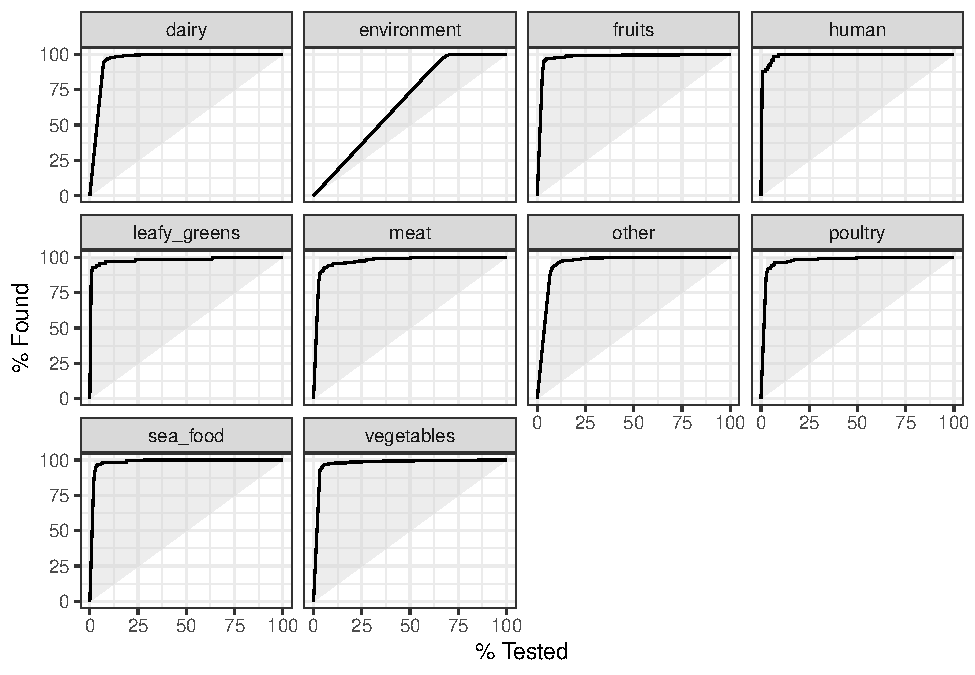
\includegraphics{php2550_final_manuscript_files/figure-latex/fig-three-1} 

}

\caption{Gain curves comparing the performance of the random forest algorithm to random guessing for all listeria pathogen isolation sources. The model shows a high gain relative to random guessing.}\label{fig:fig-three}
\end{figure}

\begin{figure}[H]

{\centering 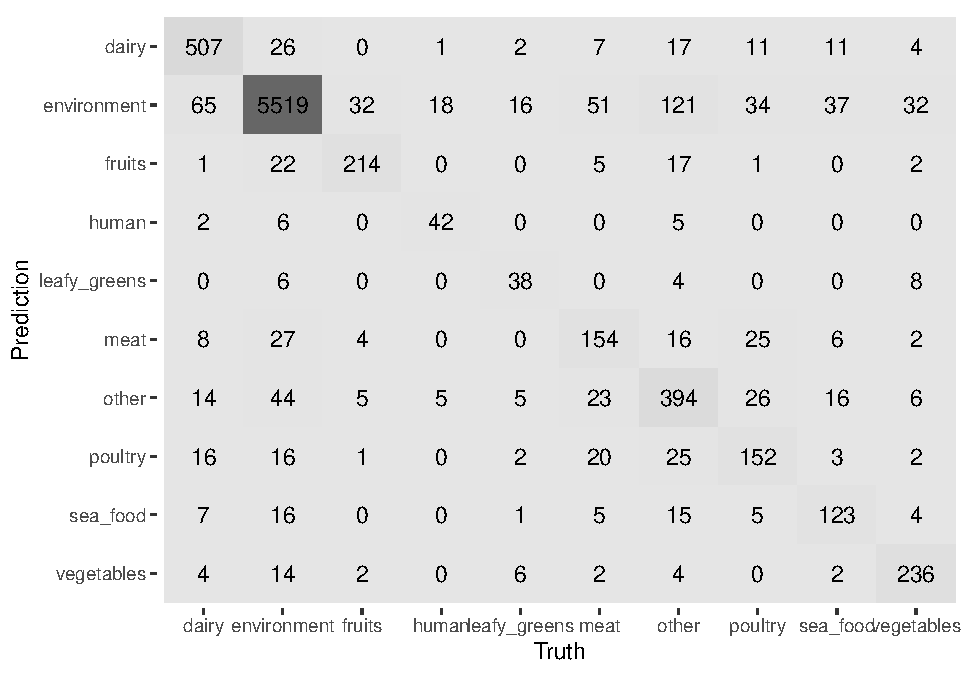
\includegraphics{php2550_final_manuscript_files/figure-latex/figure-four-1} 

}

\caption{Performance of the random forest model in $\textit{Listeria monocytogene}$ source attribution. The model showed a relatively good classification performance.}\label{fig:figure-four}
\end{figure}

\hypertarget{variable-importance}{%
\subsubsection{Variable importance}\label{variable-importance}}

Figure \ref{fig:figure-five} shows the variable importance based on the random forest algorithm and the contributions of the features employed in modeling to node purity. The most important variables in linking a listeriosis pathogen to a source based on this model were the strain, the isolate, the state from which the pathogen was collected, the minimum SNP distance to another SNP of a different type, the minimum distance to a SNP of the same type, the season of the month the pathogen was collected, and the SNP cluster.

\begin{figure}[H]

{\centering 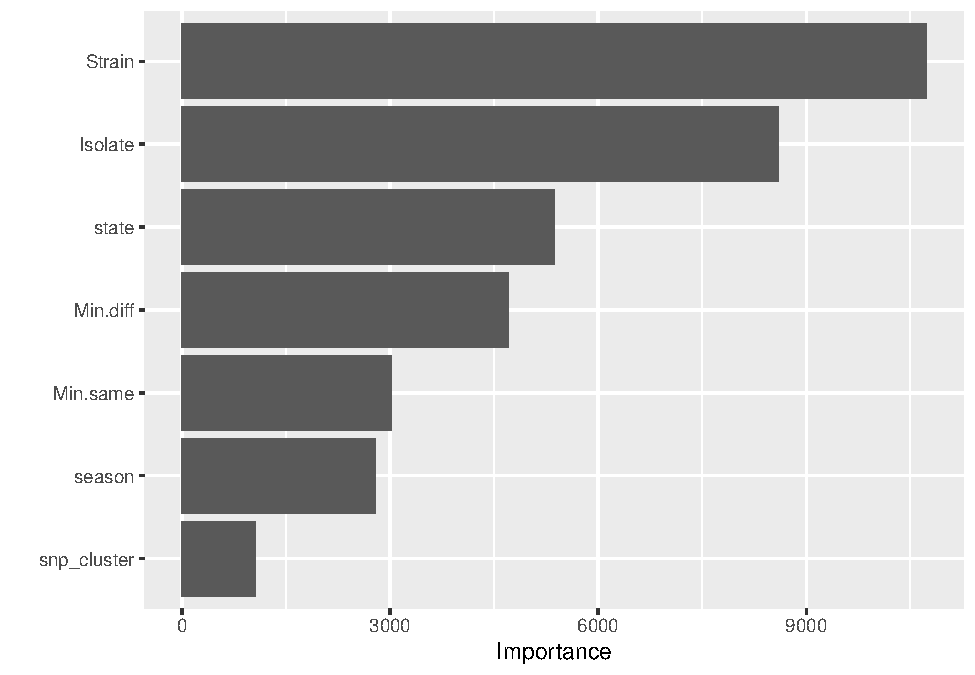
\includegraphics{php2550_final_manuscript_files/figure-latex/figure-five-1} 

}

\caption{Variable importance in the attribution of listeria pathogens to a source based on the random forest model. The strain denoting the microbial strain name used to distinguish a genetically distinct lineage separated from another strain by one or two mutations and the isolate type were the most substantial features in source attribution of listeria pathogens whereas the SNP cluster had the least significance.}\label{fig:figure-five}
\end{figure}

\hypertarget{discussion}{%
\subsection{Discussion}\label{discussion}}

Surveillance of foodborne illness plays a critical role in limiting the incidence and prevalence rates of a disease. Early detection of sources linked to outbreaks can facilitate immediate response and implementation of public health policies and intervention measures aimed at reducing the burden of a disease. This study aimed at comparing different statistical machine learning models to propose a suitable model with high accuracy and efficiency in predicting the sources of listeria pathogens using data from the NCBI pathogen detection database. Accurate identification of sources linked to listeria can result in prompt responses to listeria outbreaks, thus reducing disease prevalence and mortality. This study found that compared with the naive Bayes classification algorithm, the random forest model showed higher accuracy and discrimination ability (AUC) of 88\% and 96\%, respectively. Given the robustness to class imbalance, high accuracy, and discriminatory ability, the the random forest model performs well in source attribution of listeria monocytogenes pathogens. The study presents a simple model for linking a listeria monocytogene pathogens given features including strain, isolate type, collection location, minimum SNP distances to SNPs of the same or different type, the sample collection season, and the SNP cluster. In previous studies examining the role of machine learning methods in source attribution, the efficiency presented by these methods and their invaluable nature, particularly, to the public health practitioners, food industry professionals, microbiologists, among other professionals in allowing tailored practice has been highlighted {[}\protect\hyperlink{ref-tanui2022machine}{3}{]}. Promising performances using machine learning methods for listeriosis pathogen tracking in outbreak investigations were reported in the study by Liu et al. {[}\protect\hyperlink{ref-liu2021machine}{22}{]} who implemented the XGBoost algorithm with cgMLST profiles of L. monocytogenes.

\hypertarget{study-strengths-and-limitations}{%
\subsubsection{Study strengths and limitations}\label{study-strengths-and-limitations}}

One of the baseline and developmental objectives of Healthy People 2030 {[}\protect\hyperlink{ref-Healthypeople2030}{46}{]} is to reduce the incidence of laboratory-diagnosed, domestically-acquired \emph{Listeria monocytogenes} infections and outbreaks related to food sources such as dairy, beef, fruits, poultry and leafy greens. Existing literature support machine learning predictive-based modeling as a meaningful approach to reducing incidence of foodborne illness in the US {[}\protect\hyperlink{ref-tanui2022machine}{3}{]}, {[}\protect\hyperlink{ref-Munck2020}{18}{]}, {[}\protect\hyperlink{ref-Njage2019}{19}{]}, {[}\protect\hyperlink{ref-lupolova2017patchy}{20}{]}, {[}\protect\hyperlink{ref-liu2021machine}{22}{]}. This study offers to propose a simple and robust model to use in providing estimates of the food categories responsible for \emph{Listeria monocytogenes} pathogens by comparing the performance of the Bayesian-based Naive Bayes classification algorithm and the ensemble-based random forest algorithm. The study characterizes the importance of using \texttt{strain}, \texttt{seasonality}, \texttt{location}, \texttt{isolate} information. Additionally, the effect of minimum SNP distance from one clinical isolate to another clinical isolate or to another isolate of of a different isolation type was incorporated into the model building process. The information from the current study can help the government, risk managers and relevant departments to carry out risk inspection, food safety investigation and health risk assessment, so that they can better predict and identify potential risks. This study also deploys an interactive web-based for the prediction of a probable source of a particular isolate and gives epidemiologists and other public health practitioners a chance to interact, in real-time, and evaluate potential sources of a particular pathogen given a set of features as input.

Our study is, however, not without limitations. First, even though in this investigation explores how machine learning models can be used to aid in foodborne illness outbreak investigations, the study focuses on only one foodborne disease pathogen, that is, L. monocytogene and is thus limited in this way to only this particular isolate. Even so, the methodology employed herein can be extended to other foodborne disease pathogens available on the NCBI pathogen detection database. Secondly, this study also reflects the general limitations presented by the data source and the quality of the data therein. The NCBI pathogen detection database allows real-time identification of clusters of related genomic sequences to aid in outbreak detection, and tracks the spread of resistance genes. A potential limitation of this data source is that it does not identify outbreaks or outbreak memberships and analyses rely solely on publicly available data submitted to the database. Thirdly, given that NCBI {[}\protect\hyperlink{ref-ncbi2016}{29}{]} collects data from currently ongoing surveillance with multitude of sources such as production facilities, food, and human patients; the database allows a lot of flexibility in the naming conventions employed on the variables which results in substantial heterogeneity in reporting and data quality which makes it difficult to query and extract meaningful patterns for microbial risk assessments {[}\protect\hyperlink{ref-sanaa2019genomegraphr}{47}{]}. For instance, the \texttt{collected\ by} and \texttt{isolation\ source} are fields that were entered as free text which are very extreme in the options they present for analysis. As a result of this flexibility in this naming conventions, we were forced to re-categorize variables based on our knowledge of the database, as well as, our assessment of overall patterns in the naming conventions, a situation which might have resulted in bias due to the subjective nature of the resulting categories, and a loss in general efficiency, particularly with respect to our outcome variable.

Fourth, our study was restricted to a complete case analysis due to high percentage of missing data on potentially useful features such as those related to phenotypic strain characteristics, a scenario which made it difficult to account for this variables in our model to enhance robustness in the derivation of inferences that could inform the development of policies governing the food production industry, and ultimately reduce the incidence of foodborne illnesses. Fifth, for our analyses, the study used data from a period spanning over 20 years and did not account for the changes in listeriosis outbreaks/incidence over time. Perhaps, a shorter, more recent period would have been more desirable when major implicated food sources have changed. For example, Listeria outbreaks caused by contamination of ready-to-eat meats products remarkably decreased after 2002. Even so, the fact that our study is based on an analyses sample this large gives a higher leverage in terms of the ability of our models to learn from the patterns in this dataset over the period. Sixth, the current study only compared two models. Future studies could examine other models such as gradient boosting machine (GBM) models. In this analysis, we excluded models that proved extremely difficult to train or which which had a relatively high computational intensity needed in the hyper-parameter tuning.

\hypertarget{conclusion-and-recommendations}{%
\subsection{Conclusion and recommendations}\label{conclusion-and-recommendations}}

In conclusion, machine learning presents an effective way of deriving inference from data to inform listeriosis outbreak investigations and presents one way technology can be used to inform public health practice. In this study, we found the random forest algorithm to be particularly efficient in listeria pathogens source attribution. The robustness of the model based on our findings indicates that machine learning methods have the potential for use in environmental surveillance, risk assessment, and management programs for pathogenic source attribution. Recommendations for future work include incorporating information on outbreak data as outbreak investigations often definitively link illnesses to particular foods and pathogenic sources. Further work can compare additional machine learning models such as gradient boosting machine (GBM), Logit boost, stochastic gradient boosting and support vector machine learning models in the context of source attribution for different pathogens using genetic data. Additional validation should be carried out, perhaps using external data, to enhance the usefulness and check generalizability of the developed model for source attribution before extended utilization of the developed source attribution web portal (model) in other countries or on new data as it becomes available.

\newpage

\hypertarget{references}{%
\subsection{References}\label{references}}

\hypertarget{refs}{}
\begin{CSLReferences}{0}{0}
\leavevmode\vadjust pre{\hypertarget{ref-who2015}{}}%
\CSLLeftMargin{{[}1{]} }%
\CSLRightInline{Organization WH. Estimates of the global burden of foodborne diseases, \url{https://www.who.int/multi-media/details/estimates-of-the-global-burden-of-foodborne-diseases} (2015).}

\leavevmode\vadjust pre{\hypertarget{ref-Lee2021}{}}%
\CSLLeftMargin{{[}2{]} }%
\CSLRightInline{Lee H, Yoon Y. Etiological agents implicated in foodborne illness world wide. \emph{Food Science of Animal Resources}; 41. Epub ahead of print 2021. DOI: \href{https://doi.org/10.5851/KOSFA.2020.E75}{10.5851/KOSFA.2020.E75}.}

\leavevmode\vadjust pre{\hypertarget{ref-tanui2022machine}{}}%
\CSLLeftMargin{{[}3{]} }%
\CSLRightInline{Tanui CK, Karanth S, Njage PM, et al. Machine learning-based predictive modeling to identify genotypic traits associated with salmonella enterica disease endpoints in isolates from ground chicken. \emph{LWT} 2022; 154: 112701.}

\leavevmode\vadjust pre{\hypertarget{ref-Scallan2011}{}}%
\CSLLeftMargin{{[}4{]} }%
\CSLRightInline{Scallan E, Hoekstra RM, Angulo FJ, et al. Foodborne illness acquired in the united states-major pathogens. \emph{Emerging Infectious Diseases}; 17. Epub ahead of print 2011. DOI: \href{https://doi.org/10.3201/eid1701.P11101}{10.3201/eid1701.P11101}.}

\leavevmode\vadjust pre{\hypertarget{ref-gourama2020foodborne}{}}%
\CSLLeftMargin{{[}5{]} }%
\CSLRightInline{Gourama H. Foodborne pathogens. In: \emph{Food safety engineering}. Springer, 2020, pp. 25--49.}

\leavevmode\vadjust pre{\hypertarget{ref-chlebicz2018campylobacteriosis}{}}%
\CSLLeftMargin{{[}6{]} }%
\CSLRightInline{Chlebicz A, Śliżewska K. Campylobacteriosis, salmonellosis, yersiniosis, and listeriosis as zoonotic foodborne diseases: A review. \emph{International journal of environmental research and public health} 2018; 15: 863.}

\leavevmode\vadjust pre{\hypertarget{ref-filipello2020attribution}{}}%
\CSLLeftMargin{{[}7{]} }%
\CSLRightInline{Filipello V, Mughini-Gras L, Gallina S, et al. Attribution of listeria monocytogenes human infections to food and animal sources in northern italy. \emph{Food microbiology} 2020; 89: 103433.}

\leavevmode\vadjust pre{\hypertarget{ref-lomonaco2015evolution}{}}%
\CSLLeftMargin{{[}8{]} }%
\CSLRightInline{Lomonaco S, Nucera D, Filipello V. The evolution and epidemiology of listeria monocytogenes in europe and the united states. \emph{Infection, Genetics and Evolution} 2015; 35: 172--183.}

\leavevmode\vadjust pre{\hypertarget{ref-cdc2022}{}}%
\CSLLeftMargin{{[}9{]} }%
\CSLRightInline{Disease Control C for, Prevention. Listeria (listeriosis) \textbar{} listeria \textbar{} CDC, \url{https://www.cdc.gov/listeria/index.html} (2022).}

\leavevmode\vadjust pre{\hypertarget{ref-matle2020review}{}}%
\CSLLeftMargin{{[}10{]} }%
\CSLRightInline{Matle I, Mbatha KR, Madoroba E. A review of listeria monocytogenes from meat and meat products: Epidemiology, virulence factors, antimicrobial resistance and diagnosis. \emph{Onderstepoort Journal of Veterinary Research} 2020; 87: 1--20.}

\leavevmode\vadjust pre{\hypertarget{ref-hilliard2018genomic}{}}%
\CSLLeftMargin{{[}11{]} }%
\CSLRightInline{Hilliard A, Leong D, O'Callaghan A, et al. Genomic characterization of listeria monocytogenes isolates associated with clinical listeriosis and the food production environment in ireland. \emph{Genes} 2018; 9: 171.}

\leavevmode\vadjust pre{\hypertarget{ref-schwartz1989investigation}{}}%
\CSLLeftMargin{{[}12{]} }%
\CSLRightInline{Schwartz B, Hexter D, Broome CV, et al. Investigation of an outbreak of listeriosis: New hypotheses for the etiology of epidemic listeria monocytogenes infections. \emph{Journal of Infectious Diseases} 1989; 159: 680--685.}

\leavevmode\vadjust pre{\hypertarget{ref-chen2017prevalence}{}}%
\CSLLeftMargin{{[}13{]} }%
\CSLRightInline{Chen J-Q, Regan P, Laksanalamai P, et al. Prevalence and methodologies for detection, characterization and subtyping of listeria monocytogenes and l. Ivanovii in foods and environmental sources. \emph{Food Science and Human Wellness} 2017; 6: 97--120.}

\leavevmode\vadjust pre{\hypertarget{ref-jensen2016molecular}{}}%
\CSLLeftMargin{{[}14{]} }%
\CSLRightInline{Jensen AK, Björkman JT, Ethelberg S, et al. Molecular typing and epidemiology of human listeriosis cases, denmark, 2002--2012. \emph{Emerging infectious diseases} 2016; 22: 625.}

\leavevmode\vadjust pre{\hypertarget{ref-gaul2013hospital}{}}%
\CSLLeftMargin{{[}15{]} }%
\CSLRightInline{Gaul LK, Farag NH, Shim T, et al. Hospital-acquired listeriosis outbreak caused by contaminated diced celery---texas, 2010. \emph{Clinical infectious diseases} 2013; 56: 20--26.}

\leavevmode\vadjust pre{\hypertarget{ref-pouillot2016infectious}{}}%
\CSLLeftMargin{{[}16{]} }%
\CSLRightInline{Pouillot R, Klontz KC, Chen Y, et al. Infectious dose of listeria monocytogenes in outbreak linked to ice cream, united states, 2015. \emph{Emerging Infectious Diseases} 2016; 22: 2113.}

\leavevmode\vadjust pre{\hypertarget{ref-de2014global}{}}%
\CSLLeftMargin{{[}17{]} }%
\CSLRightInline{Noordhout CM de, Devleesschauwer B, Angulo FJ, et al. The global burden of listeriosis: A systematic review and meta-analysis. \emph{The Lancet Infectious Diseases} 2014; 14: 1073--1082.}

\leavevmode\vadjust pre{\hypertarget{ref-Munck2020}{}}%
\CSLLeftMargin{{[}18{]} }%
\CSLRightInline{Munck N, Njage PMK, Leekitcharoenphon P, et al. Application of whole-genome sequences and machine learning in source attribution of salmonella typhimurium. \emph{Risk Analysis}; 40. Epub ahead of print 2020. DOI: \href{https://doi.org/10.1111/risa.13510}{10.1111/risa.13510}.}

\leavevmode\vadjust pre{\hypertarget{ref-Njage2019}{}}%
\CSLLeftMargin{{[}19{]} }%
\CSLRightInline{Njage PMK, Henri C, Leekitcharoenphon P, et al. Machine learning methods as a tool for predicting risk of illness applying next-generation sequencing data. \emph{Risk Analysis}; 39. Epub ahead of print 2019. DOI: \href{https://doi.org/10.1111/risa.13239}{10.1111/risa.13239}.}

\leavevmode\vadjust pre{\hypertarget{ref-lupolova2017patchy}{}}%
\CSLLeftMargin{{[}20{]} }%
\CSLRightInline{Lupolova N, Dallman TJ, Holden NJ, et al. Patchy promiscuity: Machine learning applied to predict the host specificity of salmonella enterica and escherichia coli. \emph{Microbial genomics}; 3.}

\leavevmode\vadjust pre{\hypertarget{ref-karanth2022exploring}{}}%
\CSLLeftMargin{{[}21{]} }%
\CSLRightInline{Karanth S, Tanui CK, Meng J, et al. Exploring the predictive capability of advanced machine learning in identifying severe disease phenotype in salmonella enterica. \emph{Food Research International} 2022; 151: 110817.}

\leavevmode\vadjust pre{\hypertarget{ref-liu2021machine}{}}%
\CSLLeftMargin{{[}22{]} }%
\CSLRightInline{Liu Y-Y, Chen C-C. A machine learning-based typing scheme refinement for listeria monocytogenes core genome multilocus sequence typing with high discriminatory power for common source outbreak tracking. \emph{PloS one} 2021; 16: e0260293.}

\leavevmode\vadjust pre{\hypertarget{ref-vangay2014classification}{}}%
\CSLLeftMargin{{[}23{]} }%
\CSLRightInline{Vangay P, Steingrimsson J, Wiedmann M, et al. Classification of listeria monocytogenes persistence in retail delicatessen environments using expert elicitation and machine learning. \emph{Risk analysis} 2014; 34: 1830--1845.}

\leavevmode\vadjust pre{\hypertarget{ref-sun2019quantitative}{}}%
\CSLLeftMargin{{[}24{]} }%
\CSLRightInline{Sun W, Liu Y, Wang X, et al. Quantitative risk assessment of listeria monocytogenes in bulk cooked meat from production to consumption in china: A bayesian approach. \emph{Journal of the Science of Food and Agriculture} 2019; 99: 2931--2938.}

\leavevmode\vadjust pre{\hypertarget{ref-pasonen2019listeria}{}}%
\CSLLeftMargin{{[}25{]} }%
\CSLRightInline{Pasonen P, Ranta J, Tapanainen H, et al. Listeria monocytogenes risk assessment on cold smoked and salt-cured fishery products in finland-a repeated exposure model. \emph{International journal of food microbiology} 2019; 304: 97--105.}

\leavevmode\vadjust pre{\hypertarget{ref-mughini2022statistical}{}}%
\CSLLeftMargin{{[}26{]} }%
\CSLRightInline{Mughini-Gras L, Benincà E, McDonald SA, et al. A statistical modelling approach for source attribution meta-analysis of sporadic infection with foodborne pathogens. \emph{Zoonoses and Public Health}.}

\leavevmode\vadjust pre{\hypertarget{ref-lassen2016two}{}}%
\CSLLeftMargin{{[}27{]} }%
\CSLRightInline{Lassen SG, Ethelberg S, Björkman J, et al. Two listeria outbreaks caused by smoked fish consumption---using whole-genome sequencing for outbreak investigations. \emph{Clinical Microbiology and Infection} 2016; 22: 620--624.}

\leavevmode\vadjust pre{\hypertarget{ref-pires2014source}{}}%
\CSLLeftMargin{{[}28{]} }%
\CSLRightInline{Pires SM, Vieira AR, Hald T, et al. Source attribution of human salmonellosis: An overview of methods and estimates. \emph{Foodborne pathogens and disease} 2014; 11: 667--676.}

\leavevmode\vadjust pre{\hypertarget{ref-ncbi2016}{}}%
\CSLLeftMargin{{[}29{]} }%
\CSLRightInline{National Library of Medicine (US) National Center for Biotechnology Information B (MD): The NCBI pathogen detection project {[}internet{]}, \url{https://www.ncbi.nlm.nih.gov/pathogens/} (2016).}

\leavevmode\vadjust pre{\hypertarget{ref-gelman1995bayesian}{}}%
\CSLLeftMargin{{[}30{]} }%
\CSLRightInline{Gelman A, Carlin JB, Stern HS, et al. \emph{Bayesian data analysis}. Chapman; Hall/CRC, 1995.}

\leavevmode\vadjust pre{\hypertarget{ref-Chen2021}{}}%
\CSLLeftMargin{{[}31{]} }%
\CSLRightInline{Chen H, Hu S, Hua R, et al. Improved naive bayes classification algorithm for traffic risk management. \emph{Eurasip Journal on Advances in Signal Processing}; 2021. Epub ahead of print 2021. DOI: \href{https://doi.org/10.1186/s13634-021-00742-6}{10.1186/s13634-021-00742-6}.}

\leavevmode\vadjust pre{\hypertarget{ref-James2013}{}}%
\CSLLeftMargin{{[}32{]} }%
\CSLRightInline{James G, Witten D, Hastie T, et al. \href{https://doi.org/10.1007/978-1-4614-7138-7_6}{Linear model selection and regularization}. In: \emph{An introduction to statistical learning: With applications in r}. New York, NY: Springer New York, pp. 225--282.}

\leavevmode\vadjust pre{\hypertarget{ref-Hastie2009}{}}%
\CSLLeftMargin{{[}33{]} }%
\CSLRightInline{Hastie T, Tibshirani R, Friedman J. \href{https://doi.org/10.1007/978-0-387-84858-7_3}{Linear methods for regression}. In: \emph{The elements of statistical learning: Data mining, inference, and prediction}. New York, NY: Springer New York, pp. 43--99.}

\leavevmode\vadjust pre{\hypertarget{ref-Hvitfeldt2022}{}}%
\CSLLeftMargin{{[}34{]} }%
\CSLRightInline{Hvitfeldt E. \emph{Themis: Extra recipes steps for dealing with unbalanced data}, \url{https://CRAN.R-project.org/package=themis} (2022).}

\leavevmode\vadjust pre{\hypertarget{ref-kuhn2020}{}}%
\CSLLeftMargin{{[}35{]} }%
\CSLRightInline{Kuhn M, Wickham H. \emph{Tidymodels: A collection of packages for modeling and machine learning using tidyverse principles.}, \url{https://www.tidymodels.org} (2020).}

\leavevmode\vadjust pre{\hypertarget{ref-Kuhn2013}{}}%
\CSLLeftMargin{{[}36{]} }%
\CSLRightInline{Kuhn M, Johnson K. \emph{Applied predictive modeling}. 2013. Epub ahead of print 2013. DOI: \href{https://doi.org/10.1007/978-1-4614-6849-3}{10.1007/978-1-4614-6849-3}.}

\leavevmode\vadjust pre{\hypertarget{ref-emil2022}{}}%
\CSLLeftMargin{{[}37{]} }%
\CSLRightInline{Hvitfeldt E, Kuhn M. \emph{Discrim: Model wrappers for discriminant analysis}, \url{https://CRAN.R-project.org/package=discrim} (2022).}

\leavevmode\vadjust pre{\hypertarget{ref-wright2017}{}}%
\CSLLeftMargin{{[}38{]} }%
\CSLRightInline{Wright MN, Ziegler A. \href{https://doi.org/10.18637/jss.v077.i01}{{ranger}: A fast implementation of random forests for high dimensional data in {C++} and {R}}. \emph{Journal of Statistical Software} 2017; 77: 1--17.}

\leavevmode\vadjust pre{\hypertarget{ref-Metz1978}{}}%
\CSLLeftMargin{{[}39{]} }%
\CSLRightInline{Metz CE. Basic principles of ROC analysis. \emph{Seminars in Nuclear Medicine}; 8. Epub ahead of print 1978. DOI: \href{https://doi.org/10.1016/S0001-2998(78)80014-2}{10.1016/S0001-2998(78)80014-2}.}

\leavevmode\vadjust pre{\hypertarget{ref-Cohen1960}{}}%
\CSLLeftMargin{{[}40{]} }%
\CSLRightInline{Cohen J. A coefficient of agreement for nominal scales. Educational and psychological measurement. \emph{Educational and Psychological Measurement}; 20.}

\leavevmode\vadjust pre{\hypertarget{ref-Mandrekar2010}{}}%
\CSLLeftMargin{{[}41{]} }%
\CSLRightInline{Mandrekar JN. Receiver operating characteristic curve in diagnostic test assessment. \emph{Journal of Thoracic Oncology}; 5. Epub ahead of print 2010. DOI: \href{https://doi.org/10.1097/JTO.0b013e3181ec173d}{10.1097/JTO.0b013e3181ec173d}.}

\leavevmode\vadjust pre{\hypertarget{ref-Engelmann2021}{}}%
\CSLLeftMargin{{[}42{]} }%
\CSLRightInline{Engelmann B, Hayden E, Tasche D. Measuring the discriminative power of rating systems. \emph{SSRN Electronic Journal}. Epub ahead of print 2021. DOI: \href{https://doi.org/10.2139/ssrn.2793951}{10.2139/ssrn.2793951}.}

\leavevmode\vadjust pre{\hypertarget{ref-yardstick2022}{}}%
\CSLLeftMargin{{[}43{]} }%
\CSLRightInline{Kuhn M, Vaughan D. \emph{Yardstick: Tidy characterizations of model performance}, \url{https://CRAN.R-project.org/package=yardstick} (2022).}

\leavevmode\vadjust pre{\hypertarget{ref-Hand2001}{}}%
\CSLLeftMargin{{[}44{]} }%
\CSLRightInline{Hand DJ, Till RJ. A simple generalisation of the area under the ROC curve for multiple class classification problems. \emph{Machine Learning}; 45. Epub ahead of print 2001. DOI: \href{https://doi.org/10.1023/A:1010920819831}{10.1023/A:1010920819831}.}

\leavevmode\vadjust pre{\hypertarget{ref-R}{}}%
\CSLLeftMargin{{[}45{]} }%
\CSLRightInline{R Core Team. \emph{R: A language and environment for statistical computing}. Vienna, Austria: R Foundation for Statistical Computing, \url{https://www.R-project.org/} (2022).}

\leavevmode\vadjust pre{\hypertarget{ref-Healthypeople2030}{}}%
\CSLLeftMargin{{[}46{]} }%
\CSLRightInline{Healthy people 2030: Foodborne illness, \url{https://health.gov/healthypeople}.}

\leavevmode\vadjust pre{\hypertarget{ref-sanaa2019genomegraphr}{}}%
\CSLLeftMargin{{[}47{]} }%
\CSLRightInline{Sanaa M, Pouillot R, Vega FG, et al. GenomeGraphR: A user-friendly open-source web application for foodborne pathogen whole genome sequencing data integration, analysis, and visualization. \emph{PloS one} 2019; 14: e0213039.}

\end{CSLReferences}

\end{document}
